\documentclass[11pt]{article}

% Packages
\usepackage[utf8]{inputenc}
\usepackage{amsmath, amssymb, amsthm}
\usepackage{enumitem}
\usepackage{geometry}
\usepackage{fancyhdr}
\usepackage{mathtools}
\usepackage{multicol}
\usepackage{minted}
\usepackage{optidef}   % https://ctan.org/pkg/optidef
\usepackage[colorlinks=true, urlcolor=blue, linkcolor=blue, citecolor=blue]{hyperref}

% Page layout
\geometry{margin=0.75in}
\pagestyle{fancy}
\fancyhf{}
\rhead{Ian Gallagher}
\lhead{Math 207C Homework}
\rfoot{\thepage}
\setlength{\headheight}{14pt}

% Commands
\newcommand{\vep}{\varepsilon}
\DeclarePairedDelimiter\abs{\lvert}{\rvert}
\newcommand{\norm}[2]{\lVert #1 \rVert_{#2}}
\newcommand{\pvec}[1]{\begin{pmatrix}#1\end{pmatrix}}

% Environments
\newtheoremstyle{problemstyle}
  {1em} % Space above
  {1em} % Space below
  {\normalfont} % Body font
  {} % Indent amount
  {\bfseries} % Theorem head font
  {} % Punctuation after theorem head
  {\newline} % Space after theorem head
  {} % Theorem head spec

\theoremstyle{problemstyle}
\newtheorem{problem}{Problem}

% Custom commands
\newenvironment{solution}
  {\noindent\textbf{Solution}\quad}
  {\hfill$\blacksquare$\par\vspace{1em}}

% Enumerate styles
\setlist[enumerate,1]{label=(\alph*), ref=\alph*, itemsep=-0.2em, topsep=0.4em}
\setlist[enumerate,2]{label=(\roman*), ref=\roman*, itemsep=0em, topsep=0.2em}

% Title info
\title{Math 258A Challenge \#\texttt{6}}
\author{Ian Gallagher}
\date{\today}

\begin{document}

\maketitle


\section*{Problem 3}

We have the following optimization problem in standard form:
\begin{mini*}
  {x\in\mathbb{R}^2}
  {(x_1-1)^2 + x_2}
  {\label{eq:problem3}}
  {}
  \addConstraint{g_0(x) = x_1 + x_2 - 1}{=0}{}
  \addConstraint{g_1(x) = -x_1}{\le 0}{}
  \addConstraint{g_2(x) = -x_2}{\le 0}{}
\end{mini*}

\begin{solution}

\noindent Introduce multipliers $\mu \in\mathbb{R}$ for the equality condition and $\lambda_1,\lambda_2\ge 0$ for the inequality conditions.
The Lagrangian is:
\[
\mathcal{L}(x,\lambda,\mu)
=\,(x_1-1)^2 + x_2
+\mu\bigl(x_1+x_2-1\bigr)
-\lambda_1 x_1 - \lambda_2 x_2 .
\]

\noindent Applying the KKT conditions, we know that any optimal point must satisfy the stationarity and complementarity conditions.
Since the given problem and feasible region is convex, the KKT conditions are both necessary and sufficient for optimality.
That is, a point $x^\star$ is optimal if there exists $\lambda^\star,\mu_1^\star,\mu_2^\star\ge 0$ such that
\begin{align*}
\nabla_x \mathcal{L}(x^\star,\lambda^\star,\mu^\star) &= 0,  &&\text{(stationarity)}\\
g_0(x^\star) &= 0,                         &&\text{(primal feasibility)}\\
g_i(x^\star) &\le 0,\ i=1,2,               &&\text{(primal feasibility)}\\
\lambda_i^\star &\ge 0,\ i=1,2,            &&\text{(dual feasibility)}\\
\lambda_i^\star g_i(x^\star) &= 0,\ i=1,2. &&\text{(complementary slackness)}
\end{align*}

\noindent We can start by computing the gradient of the Lagrangian with respect to $x$:
\[
\nabla_x \mathcal{L} =
\begin{pmatrix}
2(x_1-1)+\mu - \lambda_1\\
1 + \mu - \lambda_2
\end{pmatrix}=0.
\]

\noindent The feasible set is the line segment from $(1,0)$ to $(0,1)$. There are therefore three cases to consider:
\begin{enumerate}
  \item $x_1>0,x_2>0$\label{case:1}
  \item $x_1=1,x_2=0$\label{case:2}
  \item $x_1=0,x_2=1$.\label{case:3}
\end{enumerate}

\noindent For (a), complementarity gives $\lambda_1 = 0$ and $\lambda_2 = 0$. Then we must have $\mu = -1$ and $x_1 = 1.5$ for stationarity, but this point is outside the feasible set.

\noindent For (b), the complementarity condition means $\lambda_1 = 0$. Then stationarity gives $\mu = 0$ and $\lambda_2 = 1$. All KKT conditions are satisfied, so $(1,0)$
is an optimal point.

\noindent For (c), the complementarity condition means $\lambda_2 = 0$. Then stationarity gives $\mu = -1$ and $\lambda_1 = -1$.
This does not satisfy the dual feasibility condition for $\lambda_1$, so $(0,1)$ is not an optimal point.

\noindent Therefore, the only optimal point is $(1,0)$ and we are done. A graph of the feasible set and the objective function is shown below.
\end{solution}

\begin{figure}[h]
  \centering
  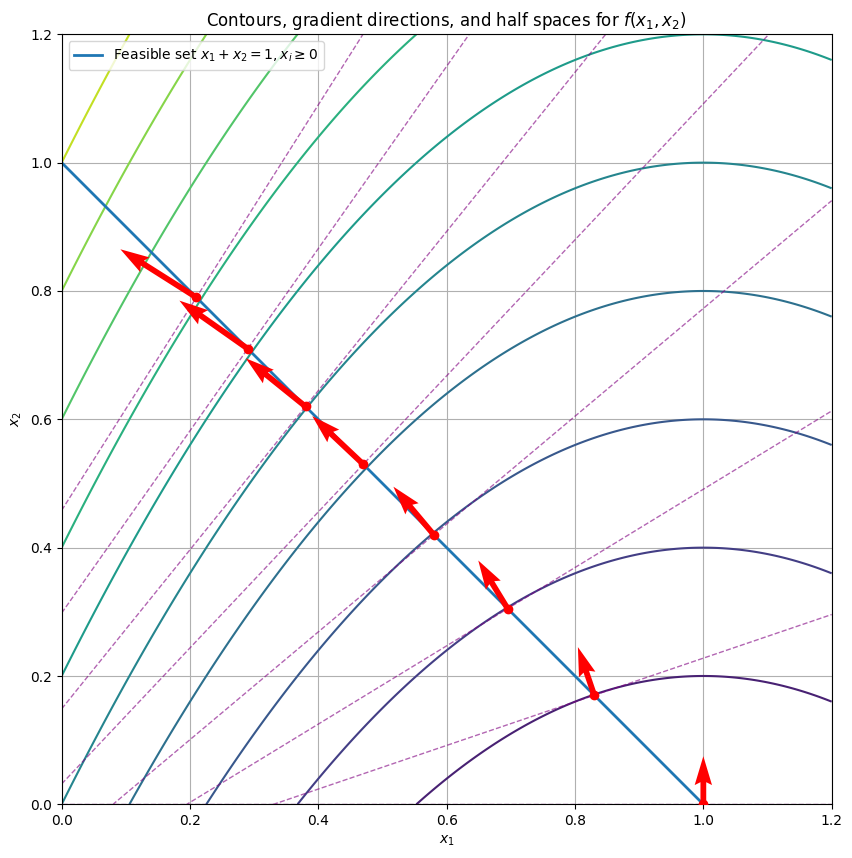
\includegraphics[width=0.8\textwidth]{contour_and_gradients.png}
  \caption{A plot of the feasible set, along with contour lines, gradient directions, and supporting planes of the objective function.}
  \label{fig:problem3}
\end{figure}


\end{document}

